\chapter{实验结果及指标分析}\label{chap:shiYan}

		\section{图像评价的客观指标}对图像质量的客观指标分为主观评价和客观评价。主观评价即这幅图片给人的视觉效果较好,使大多数人的主观感受感到舒适。而客观评价也是必不可少的,是一个算法是否有效的重要依据。但是由于不同种类的图像具有不同的特性,并且由于工程任务的目标的不同,即使是对同一种类的图像也可能提出不同的要求,因此很难有一种客观评价指标是适用于大多数图片的。本文使用图像灰度均值,图像灰度标准差,图像信息熵以及图像灰度直方图作为图像客观评价指标。将多种指标放在一起进行比较。以证明本文方法的有效性以及与其他方法的异同。
			\subsection{灰度均值}图像灰度均值表示图像的整体亮度,是一个宏观指标,是图像亮度给人的第一视觉感觉的客观反映。当图像均值一直在灰度值为128的地方小范围波动时,大多数情况下图像具有较好的视觉效果,但是例如当图像在雾天拍摄时所得的图像,不符合上述规律。图像灰度均值的计算公式如下:
\begin{equation}	u= \frac{1}{WH} \sum \sum R(x,y) 	\end{equation}	
	
此处,$WH$为图像尺寸的乘积,即宽度$W$与$H$相乘。

			\subsection{灰度标准差}图像标准差反映了图像像素灰度值与均值的离散程度,标准差越大说明图像各个像素点灰度值之间的离散化程度越高,其数学表达式为:
\begin{equation}	 	\sigma =  \sqrt{ \frac{1}{WH} \sum \sum R(x,y-u)^2}	\end{equation}

图像的灰度值标准差表示图像的的亮暗范围,标准差数值越大即表明图片所显示的亮暗范围越大。
			\subsection{图像信息熵}图像信息熵是一种统计形式,用以对图像中的平均信息量的大小进行量化。信息熵即衡量信息量的指标,信息熵满足三条性质:单调性即发生概率越高的事件所携带的信息熵越低,非负性即信息熵不能为复数和累加性。简单的说,就是信息熵是按平均概率发生一个事件观察者能得到的信息量的大小。在数学上,信息熵就是信息量的期望。图像信息熵分为一维灰度信息熵和二维灰度信息熵。其中一维灰度信息熵无法反应信息在图像二维空间上分布的特征。因此本文的图像信息熵特指二维灰度信息熵。图像信息熵的大小和图像所单位面积内包含的信息量的大小成正相关,即图像信息熵越大,图像单位面积所包含的信息量的大小越大。图像信息熵的数学表达为:
\begin{equation}	 	P = - \sum p_iln(p_i)		\end{equation}

其中,求和的范围为从灰度值的最低值到灰度值的最高值,$p_i$代表每个灰度级的概率。

		\section{实验结果}本问提出的算法是对航空图像进行增强处理,因此要充分考虑到恶劣状况对航空图像的影响。因此我们挑选两类图片进行实验,分别用直方图均衡、SSR算法和DWT—SVD算法对他们进行处理,并对结果进行分析和比较。
			\subsection{第一组实验}第一组实验对具有整体低对比度,整体偏白的特征的图片进行增强处理,即对在雾天条件下拍摄的图片进行处理。

\begin{figure}[!htbp]
    \centering
    \begin{subfigure}[b]{0.5\textwidth}
      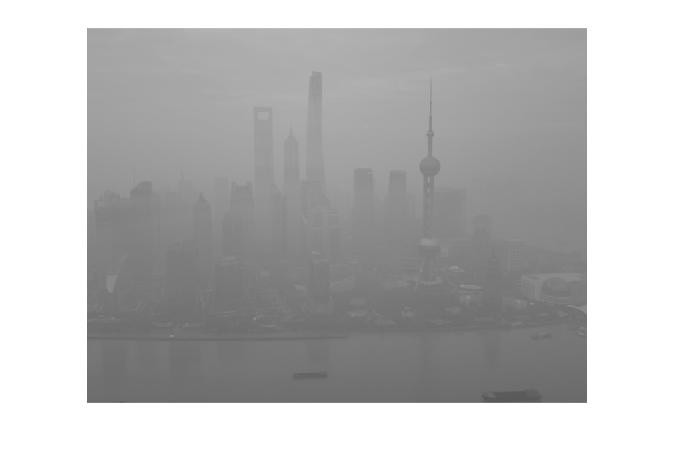
\includegraphics[width=\textwidth]{oriImg11}
      \caption{}
      \label{fig:oaspl_a}
    \end{subfigure}%
    ~%add desired spacing
    \begin{subfigure}[b]{0.5\textwidth}
      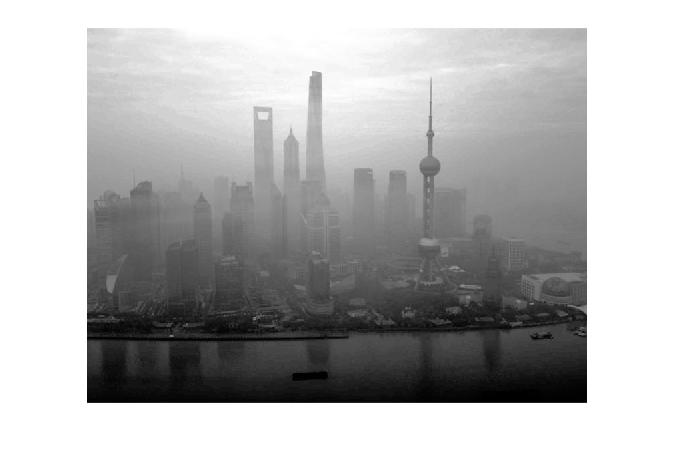
\includegraphics[width=\textwidth]{HE11}
      \caption{}
      \label{fig:oaspl_b}
    \end{subfigure}
    \begin{subfigure}[b]{0.5\textwidth}
      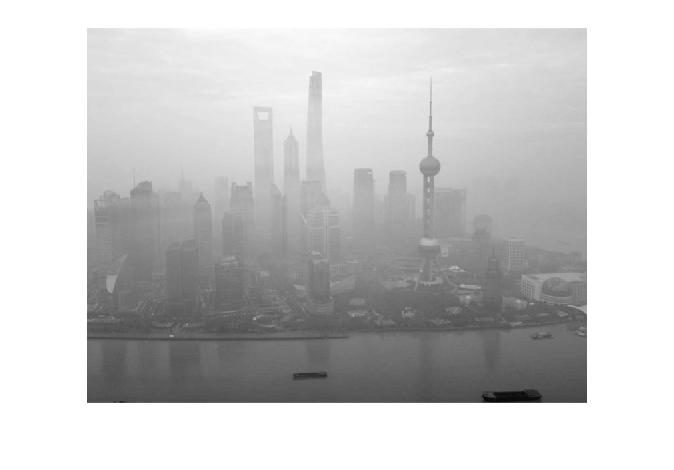
\includegraphics[width=\textwidth]{SSR11}
      \caption{}
      \label{fig:oaspl_c}
    \end{subfigure}%
    ~%add desired spacing
    \begin{subfigure}[b]{0.5\textwidth}
      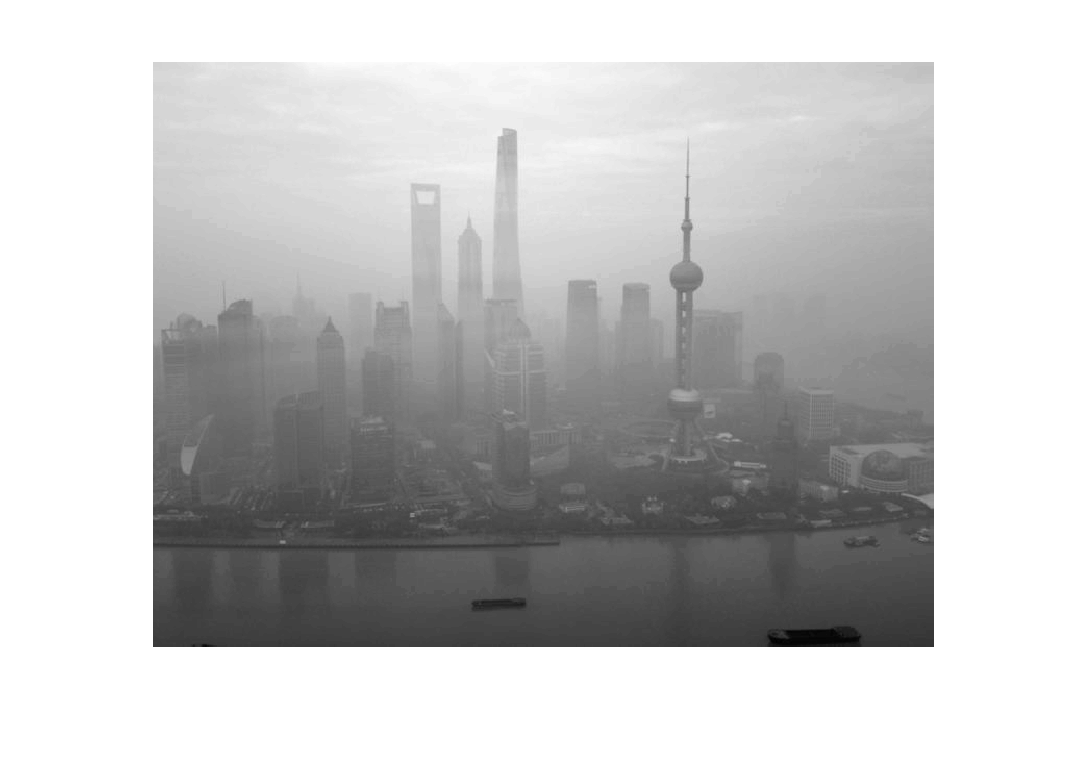
\includegraphics[width=\textwidth]{DWTSVD11}
      \caption{}
      \label{fig:oaspl_d}
    \end{subfigure}
    \bicaption{总声压级。(a) 这是子图说明信息,(b) 这是子图说明信息,(c) 这是子图说明信息,(d) 这是子图说明信息。}{OASPL.(a) This is the explanation of subfig, (b) This is the explanation of subfig, (c) This is the explanation of subfig, (d) This is the explanation of subfig.}
    \label{fig:oaspl}
\end{figure}

主观上分析,可以从图$4.1$中看出原图像的特点为:图像整体模糊不清,近景的物体依稀可见有一条和几条船,远景的物体是一些看不清楚但是可以逻辑判断出的建筑物,但是城市中的道路和建筑轮廓人眼难以辨认。直方图均衡算法增强后的图像整体视觉效果更好,并且城市中的道路和建筑轮廓清晰可辨,但是存在过增强的缺点。例如此图片右下角呈现出全黑的局部图象,但是原图中可以看见有一只小船。单尺度Retinex算法增强后的图像右下角有船只即没有展现出过增强的迹象,也实现了去雾的效果,但是部分细节不如直方图均衡算法的结果清晰。总体而言,单尺度Retinex算法的效果比直方图均衡的效果在雾天航空图像上来的好。而DWT-SVD增强算法的主观效果整体相差不大,但在局部,例如城市中的建筑轮廓与背景比较,DWT-SVD算法的结果更加清晰,更好的改善视觉效果。

\begin{table}[!htbp]
    \bicaption{客观指标}{objective indicator}
    \label{tab:sample}
    \centering
    \footnotesize% fontsize
    \setlength{\tabcolsep}{4pt}% column separation
    \renewcommand{\arraystretch}{1.2}%row space 
    \setlength{\tabcolsep}{7mm}{
    \begin{tabular}{|r|r|r|r|}
	  \hline
        算法   			   & 均值 & 标准差 & 信息熵 \\
	\hline
	   原始   			   & $140.48$ & $21.35$ & $6.07$ \\
	\hline
        直方图均衡            & $129.61$ & $73.47$ & $6.04$ \\
	\hline
        SSR算法			    & $163.49$ & $53.24$ & $7.19$ \\
	\hline
        DWT-SVD算法       & $147.93$ & $58.64$ & $7.47$ \\
        \hline
    \end{tabular}}
    
\end{table}


从客观指标来看,可以从表格中看出,四幅图片的均值都偏高图像整体显示出白色,增强算法增强后的结果图的标准差数值大小普遍偏大,在一定程度上说明图像质量较好,而在图像信息熵方面增强算法增强后的图像的数值比原图像的数值大,也说明这三种的算法的有效的增加了原图像的信息量,其中DWT-SVD算法最为出众,其次是SSR算法。

			\subsection{第二组实验}第二组实验对具有整体对比度偏低,其中部分地方偏白的特点,拍摄场景为在薄雾天气,阳光较为强烈的条件下拍摄。


\begin{figure}[!htbp]
    \centering
    \begin{subfigure}[b]{0.5\textwidth}
      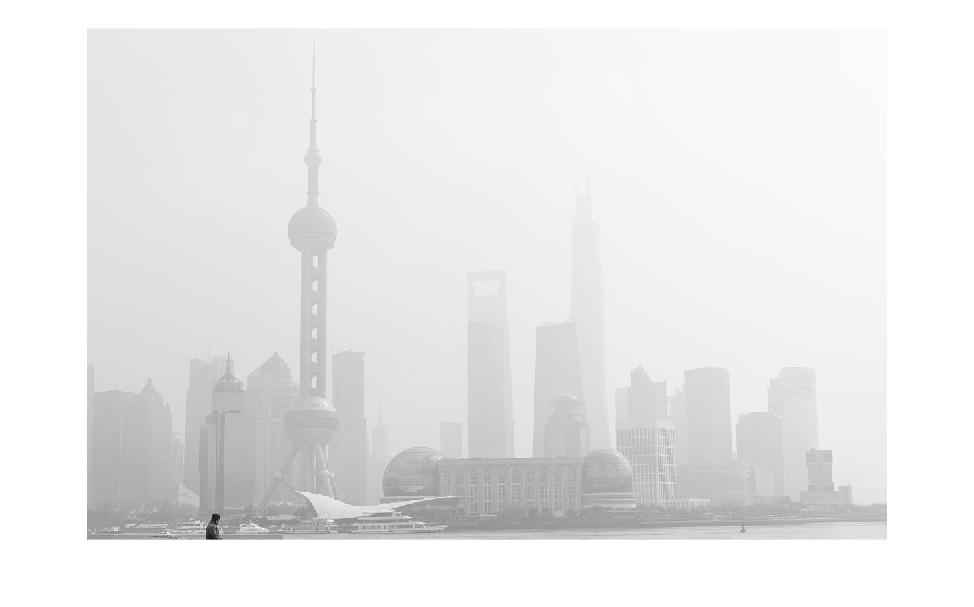
\includegraphics[width=\textwidth]{oriImg16}
      \caption{}
      \label{fig:oaspl_a}
    \end{subfigure}%
    ~%add desired spacing
    \begin{subfigure}[b]{0.5\textwidth}
      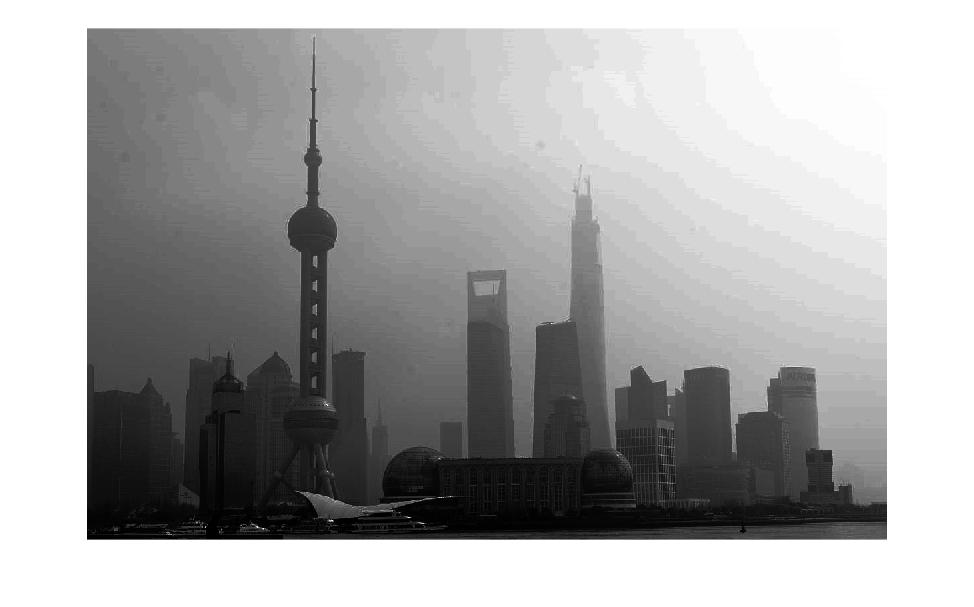
\includegraphics[width=\textwidth]{HE16}
      \caption{}
      \label{fig:oaspl_b}
    \end{subfigure}
    \begin{subfigure}[b]{0.5\textwidth}
      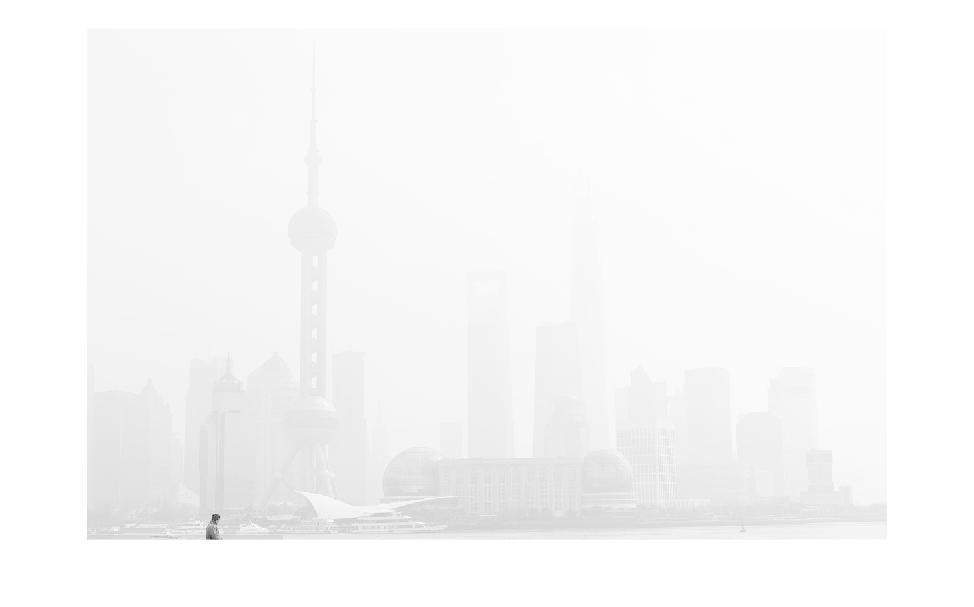
\includegraphics[width=\textwidth]{SSR16}
      \caption{}
      \label{fig:oaspl_c}
    \end{subfigure}%
    ~%add desired spacing
    \begin{subfigure}[b]{0.5\textwidth}
      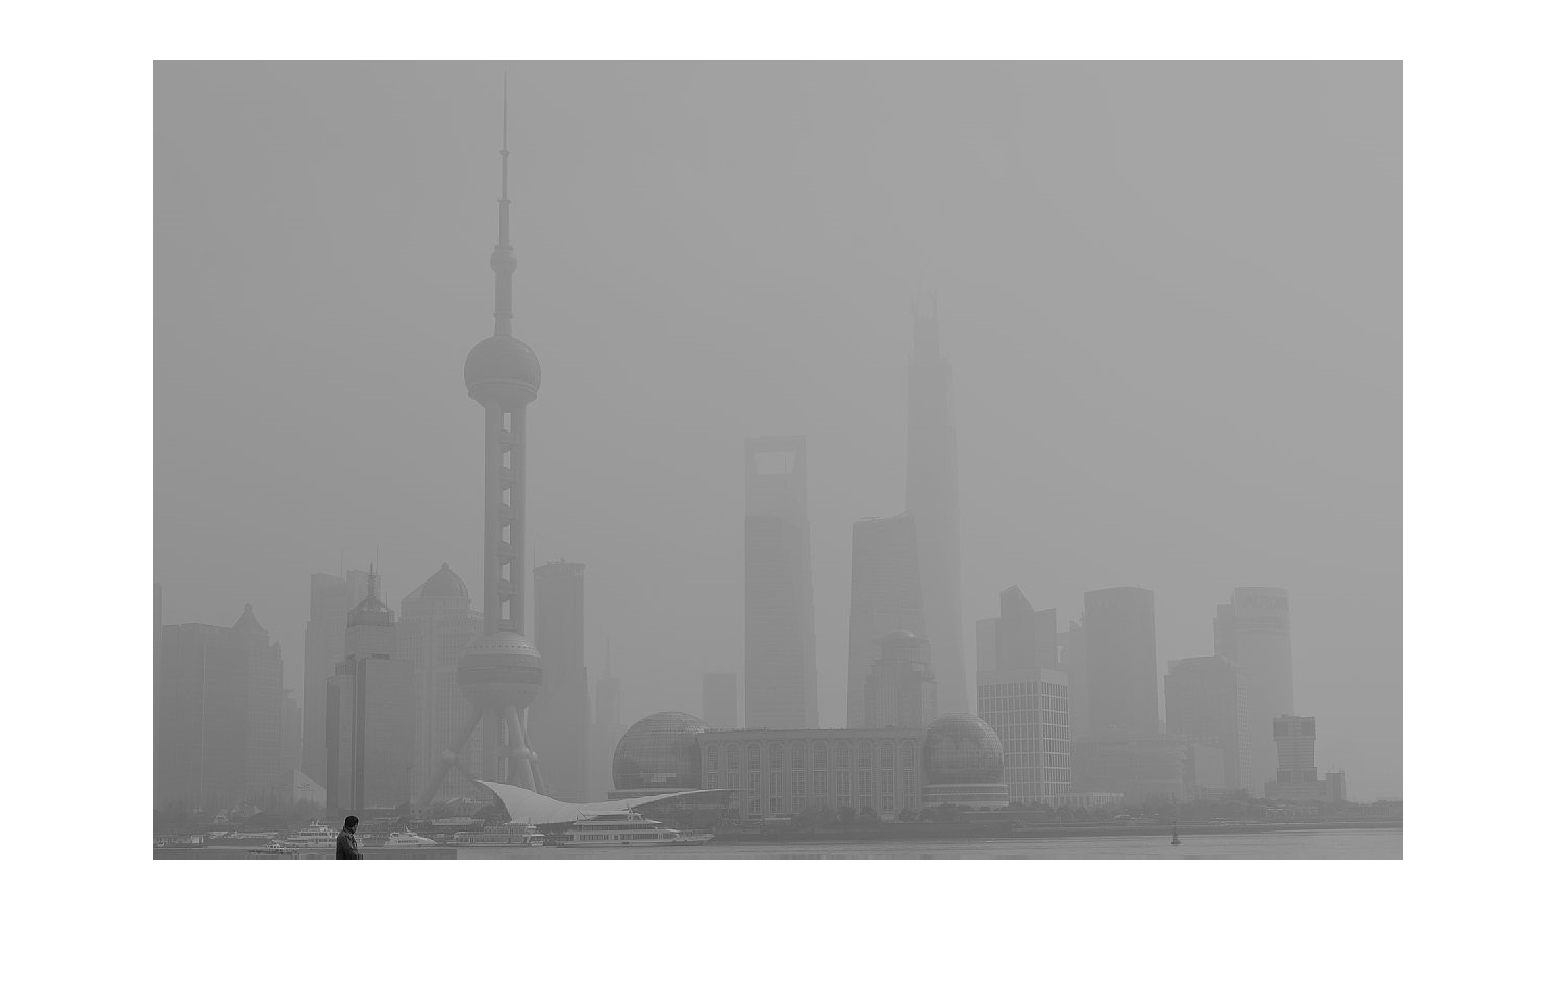
\includegraphics[width=\textwidth]{DWTSVD16}
      \caption{}
      \label{fig:oaspl_d}
    \end{subfigure}
    \bicaption{总声压级。(a) 这是子图说明信息,(b) 这是子图说明信息,(c) 这是子图说明信息,(d) 这是子图说明信息。}{OASPL.(a) This is the explanation of subfig, (b) This is the explanation of subfig, (c) This is the explanation of subfig, (d) This is the explanation of subfig.}
    \label{fig:oaspl}
\end{figure}

图4.2中直方图均衡算法造成了多处地方细节丢失,但也有让观察者更清楚的看清楚建筑轮廓的优点,而SSR算法效果不理想整体偏白,看不清细节,图像效果不如原图,SSR算作作为一种经典的去雾算法在此种场景并不适用。DWT-SVD算法图像效果和原图相差不大,但是在此类图像上的整体效果显然优于直方图均衡和SSR算法增强后的结果。

\begin{table}[t!]
    \bicaption{客观指标}{objective indicator}
    \label{tab:sample}
    \centering
    \footnotesize% fontsize
    \setlength{\tabcolsep}{4pt}% column separation
    \renewcommand{\arraystretch}{1.2}%row space 
    \setlength{\tabcolsep}{7mm}{
    \begin{tabular}{|r|r|r|r|}
	  \hline
        算法   			   & 均值 & 标准差 & 信息熵 \\
	\hline
	   原始   			   & $223.61$ & $24.39$ & $6.10$ \\
	\hline
        直方图均衡            & $129.94$ & $74.94$ & $6.03$ \\
	\hline
        SSR算法			    & $244.36$ & $9.37$ & $4.57$ \\
	\hline
        DWT-SVD算法       & $148.39$ & $16.33$ & $6.23$ \\
        \hline
    \end{tabular}}
    
\end{table}



